\documentclass[11pt]{article}
\usepackage[cp1251]{inputenc}
\usepackage[bulgarian,english]{babel}
\usepackage[LGR,X2,T1]{fontenc}
\usepackage[T2A]{fontenc}
\usepackage{graphicx}

\begin{document}
\selectlanguage{bulgarian}
\textwidth 135mm
\textheight 194mm
\begin{center}
{\large \textbf{ПРОЕКТЪТ \textit{МЕЙКАМП АРЕНА} -- ИЗПОЛЗВАНЕ НА
СЪСТЕЗАТЕЛНИ СИСТЕМИ В ОБУЧЕНИЕТО ПО ПРОГРАМИРАНЕ}}\footnote{This
work is partly supported by Scientific Research Fund of Sofia
University under the Contract 247/2010.}

\vspace*{5mm}

\textbf{Валентин Михов}

\end {center}

\vspace*{5mm}
\parbox{11,7cm}{\footnotesize
Състезателните системи (СС) са съществен инструмент в
органи\-зацията на състезания по програмиране за ученици и студенти.
Днес няма състезание по програмиране на международно ниво, което да
не използва СС, а националните състезания, неизполз\-ващи
състезателни системи са все по-малко. Настоящата статия описва една
възможност за използване на СС в процеса на обучението по
програмиране и подготовка на състезатели, реализирана в рамките на
проекта \textit{Мейкамп}. }

\vspace*{5mm}

\textbf{1. Състезателните системи.} Подробно описание на
състезателните системи (СС) - предназначение, архитектура, основни
функции и т.н., може да бъде намерено в [1], затова тук ще се спрем
съвсем накратко на техните характеристики. Всяка СС (на английски
Grading system или прсто Grader), по своята същност представлява
софтуерна система, която предоставя на участниците в състезания по
програмиране възможност да изпращат решенията на състезателните
задачи (изходен код на програма, написан на един от езиците за
програмиране поддържани от системата). Системата архивира
изпратеното решение, компилира го до изпълним код и проверява дали
получената програма решава поставената задача, като изпълнява
програмата върху зададено множество от тестове, в рамките на
поставени ограничения за време и памет, и сравнява получените
резултати с очакваните.

Това разбира се е доста опростено описание на същността на СС, тъй
като в повечето случай една СС трябва да предоставя възможност за
организиране на състезания по програмиране, за съхранение и
визуализиране на условията на задачите, за генериране на класиране,
поддръжка на различни видове задачи и оценявания и т.н. СС са
изключително полезни при организирането на състезания по
програмиране, тъй като автоматизират напълно тестването на
решенията. Без използването на СС, тестването на програмите на
състезателите се извършваше ръчно и отнемаше много време. Освен това
СС може да автоматизира и други дейности, като генериране на
класирания, статистики и архиви на състезанията.

Една от първите състезателни системи е системата $PC^2$, днес
официална състезателна система на ACM ICPC -- Международната
олимпиада по програмиране за студенти [2]. От 2000 година
Международните олимпиади по информатика за ученици също използват
състезателни системи, създавани обикновено от страната домакин. В
организираните в България състезания по програмиране -- както
национални, така и международни -- се използват системите SMOC [3] и
spoj0 [4].

Практиката отдавна е показала, че СС са незаменим помощник за
организаторите на състезания по програмиране. Интересното е, че не е
толкова очевидно как една такава система може да помогне в
обучението на ученици и студенти по програмиране. Има примери на СС,
които се използват в процеса на обучение по програмиране. В [5]
авторите описват опита си в прилагане на СС в обучението по
програмиране в Португалия. Системата spoj0 се използва активно във
Факултета по математика и информатика на Софийския университет при
преподаване на курсове по алгоритми. Елементи на обучение предлага,
например, системата USACO за подготовка на американските ученици,
които се готвят за участие в Международната олимпиада по
програмиране [6].

За съжаление, споменатите системи не са много популярни сред
учениците в България, особено сред по-малките. Това се дължи до
голяма степен на факта, че тези системи са ``затворени'' в рамките
на съответните институции или за използването им е необходимо добро
владеене на чужд език (най-често английски), което прави
използването им от по-малки ученици трудно или невъзможно.

Разглежданият в тази статия проект има за цел да подпомогне
подготовката на начинаещи програмисти с използване на състезателна
система. В раздел 2 е представена една ранна фаза на проекта и някои
негови недостатъци. В раздел 3 са формулирани проектните идеи, които
трябваше да ни приближат по близко да целта на проекта. В раздел 4
са представени някои резултати от едногодишната работа на сайта, а в
раздел 5 - насоки за бъдещи усъвършенствания.

\textbf{2. Проектът \textit{Мейкамп}.} Първоначално идеята на
проекта Мейкамп беше да се създаде Интернет сайт, който да помага на
учениците от българските училища в обучението им по информатика,
както и да се мотивират учениците да се занимават сериозно със
състезания по програмиране.

През първата година на осъществяването на проекта бяха изготвени
редица видео-лекции по важни теми в областта на информатиката, както
и задачи за упражнение. Лекциите бяха диференцирани по теми, като
например \textit{Графи}, \textit{Динамично програмиране}, и т.н. В
края на всяка видео-лекция се предлагаше списък от задачи, които
слушателите трябваше да решат сами. Учениците, които изявиха желание
да участват в предложената форма на обучение, бяха разпределени
между няколко опитни програмисти -- \textit{ментори}, които от близо
следяха прогреса на състезателите и работеха директно с тях, когато
имаха нужда от помощ.

След една година работа с този модел на подготовка, бяха отчетени
някои негови отрицателни страни:

\begin{enumerate}
\item
Моделът беше трудно скалируем и включването на повече ученици в
занятията практически невъзможно;

\item
Учениците, които успяваха да участват сериозно в подготовката през
цялото време бяха много малко;

\item
След няколко месеца прилагане на модела, повечето участващи ученици
бяха на мнение, че това което им липсва е повече практика в реални
състезания.
\end{enumerate}

След като проведохме анкета сред участниците установихме, че
повечето ученици смятат, че изключително полезно за тяхната
подготовка би било, ако на Интернет сайта на проекта се организират
състезания, наподобяващи състезанията на национално ниво по
същността на предлаганите задачи и времетраене. Нашият опит като
бивши състезатели по информатика също подсказваше, че това може би
ще помогне повече от колкото видео-лекциите. Така една година след
започване на работата по проекта \textit{Мейкамп}, беше решено да се
смени посоката на развитие и да се организира сайт, на който да се
провеждат състезания.

Беше решено да се организират състезания с различни нива на
трудност, за да могат да участват както опитни състезатели, така и
ученици, които имат малък опит или тепърва започват своя път в
състезателната информатика. В стратегията на \textit{Майкамп} е
дълбоко застъпена идеята, че малките ученици са най-важни, тъй като
измежду тях ще се търсят тези, които имат потенциала да израснат
като състезатели, а най-опитните състезатели обикновено са
достатъчно мотивирани за да могат да тренират и да се подготвят
сами.

\textbf{3. Изграждане на \textit{Мейкамп Арена}.} Преди да започнем
да разработваме сайта \textit{Мейкамп Арена}, предназначен за
провеждане на състезания по програмиране, формулирахме няколко
основни цели, които искаме да постигнем. В съответствие с
поставените цели бяха взети и съответните проектни решения за
изграждането на сайта. По-долу са представени тези решения, с кратко
описание на основанията за съответното решение.

\textit{\textbf{3.1. Нива на трудност.}} За да е полезен сайтът за
възможно най-широк кръг от състезатели беше решено, така както в
системата USACO, състезания да се организират в 3 дивизии с различно
ниво на трудност, както следва:

\begin{itemize}
\item
\textit{Златна дивизия} с високо ниво на трудност -- на нивото на
Международната олимпиада по информатика и на последния кръг на
Националната олимпиада по информатика. Тази дивизия е съответна на
състезателната група A от националните състезания;

\item
\textit{Сребърна дивизия} със средно ниво на трудност. Дивизията
предназначена за състезатели, които все още не са достигнали нивото
в златната дивизия, но им трябва още малко практика за да го
достигнат. Тази дивизия е съответна на състезателната B група
от националните състезания;

\item
\textit{Бронзова дивизия} е с най-ниско ниво на трудност.
Предназначена е за начинаещи състезатели, които  прохождат в
състезателната информатика и тепърва им предстои да участват в
състезания. Това по същество са учениците от групите C, D и Е на
националните състезания. Идеята е да им се създадат условия подобни
на тези, с които ще се сблъскат по време на националните състезания,
за да натрупат достатъчно състезателен опит и знания.

\end{itemize}

\textit{\textbf{3.2. Формат на състезанията.}} Състезанията
\textit{няма да имат фиксирано начало}, но ще имат \textit{фиксирана
продължителност}, както е в USACO. В рамките на няколко дни,
опеделени за провеждане на състезанието, всеки състезателят може да
избере произволен непрекъснат интервал от време, с дължина
определена от правилата и да се опита да реши задачите в този
интервал. Така учениците ще имат гъвкавостта да изберат кога точно
ще правят състезанието, което много от тях смятат за голям плюс, тъй
като графикът на всеки ученик е различен. Освен това сайтът предлага
и \textit{тренировъчни сеанси} (\textit{практика}), каквато всеки
състезател може да си организира сам.

Оценяването ще е в \textit{два режима}. Единият режим е
\textit{оценяване в състезателен режим}. В този режим всяко
изпратено решение ще се тества с 1 тест веднага, за да са сигурни
състезателите, че решението им се компилира и изпълнява в системата.
Oценяването в този режим се извършва след приключване на
състезанието, когато се пускат останалите тестове и се вижда за колко точки работи решението. Другият е \textit{оценяване в режим на практика},
когато решенията ще се тестват с всички предвидени тестове веднага и
потребителя може да види веднага оценката на решението, което е
изпратил. Тук е важно да се отбележи, че за разлика от повечето
чуждестранни системи, \textit{Мейкамп Арена} оценява състезателите
по правилата на ученическите състезания, т.е. решението получава
оценка, пропорционална на броя тестове, за които работи вярно.

\textbf{\textit{3.3. Архиви и съпътстваща документация.}} Задачите
от състезанията се съхраняват в \textit{архив} за да могат да се
използват в тренировъчни сесии. Това е много важно, тъй като
позволява на учениците да си изберат подходяща задача за решаване и
да проверяват дали са усвоили определен алгоритъм или подход. Ако
един състезател не използва системата, то трябва за всяка една
задача, с която тренира да намери тестове и ръчно да провери
правилността на решението си.

За всяка задача се опитваме да публикуваме \textit{анализ на
решението}, също както това се прави за националните състезания по информатика [7]. Анализите на решенията са много полезни за по-малките
състезатели. За съжаление, това е изискването, което е реализирано в
най-малка степен. Към този момент не всички задачи имат анализи и
това се дължи на сложността на изготвянето на един анализ. Повечето
задачи в архива на \textit{Мейкамп Арена} са взети от различни
състезания наготово, докато анализите се изготвят от членовете на
проектния екип. А изготвянето на качествен анализ отнема доста време
и изисква сериозен опит.

\textbf{\textit{3.4. Класиране и рейтинги.}} Освен
\textit{класирането от състезания}, сайтът поддържа и
\textit{класиране от тренировъчните сесии}. Идеята е, че
състезателите трябва да се стимулират по всякакъв начин да
практикуват повече, а въвеждането на състезателен елемент в
тренировките би трябвало да стимулира учениците да се упражняват
повече. Една друга възможност за стимулиране е поддържането на
\textit{рейтинг на състезателите} в различните дивизии, какъвто
\textit{Мейкамп Арена} също предлага. Очевидно е, че могат да се
търсят и други начини за стимулиране на учениците.

\textbf{\textit{3.5. Интерфейс на съставителите на състезания.}}
Съставянето на състезания трябва да е много лесно удобно за
потребителите-треньори. При работата над \textit{Мейкамп Арена} се
опитахме да вложим опита си, който имаме с изграждането на
потребителски интерфейси и да направим сайта възможно най-лесен за
ползване. В момента създаването на ново състезание става с попълване
на една екранна форма и прикачването по един архив за всяка една
задача. Архивът трябва да съдържа условието и тестове на задачата,
подготвени в зададен формат.

Формулираните в предния раздел решения бяха имплементирани и сайтът
[8] беше публикуван за всеобщо ползване в края на 2009 г. За
прототип на СС система беше използван клонинг на системата spoj0,
приспособен за нашите цели. Началната версия на сайта вече една
година е на разположение на учениците и вече можем да направим
някаква оценка на постигнатото.

\textbf{4. Резултати.}

Едногодишното използване на сайта \textit{Мейкамп Арена} ни
позволява да очертаем някои тенденции, съобразяването с които да ни
позволи да го усъвършенстваме. Едни от първите инициативи, които
организирахме на сайта бяха тренировъчните сесии със задачи от
националните състезания. До момента сме публикували всички национални
състезания, проведени през 2010. Статистиката за броя изпратени
решения за всяко едно състезание показва (Фиг. 1), че
най-популярните състезания са именно тренировки със задачи от
националните състезания. Това ни кара да вярваме, че една такава
система помага изключително много на състезателите в израстването
им. Практикуването със задачи, които състезателите не са успели да
решат по време на състезание е услуга, която им позволява по удобен
начин да попълнят празноти в подготовката си.

\begin{figure}[h]
\begin{center}
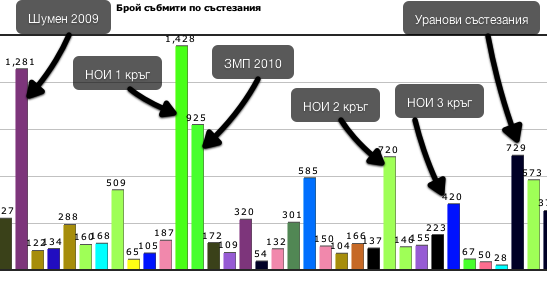
\includegraphics[width=1.0\textwidth]{contest_stats_small.png}
\end{center}
\caption{Пратени решения за всяко състезание} \label{contest_stats}
\end{figure}

Другата интересна тенденция, която се забелязва е създаването по
инициатива на преподаватели на четвърта дивизия -- \textit{Уранова}
-- предназначена за най-малките. Последните две състезания в
урановата дивизия се радват на изключителен успех. Това е резултат
на няколко фактора: тези състезания се подготвят от професионални
учители по информатика и са с изцяло авторски задачи. Не без
значение, разбира се, е и популяризацията на сайта сред най-малките
и поощряването на участниците от страната на учителите.

И малко статистика. \textit{Мейкамп Арена} започна да функционира на
14 Ноември 2009. От тогава до сега (12 Ноември 2010) са изпратени
13063 решения, което прави по 36 изпратени решения на ден.
Публикувани са 225 задачи, разпределени в 48 състезания. Има
регистрирани 489 потребителя от 45 различни града. Най-интересното
е, че в системата има няколко регистрирани потребителя от чужбина.

\textbf{5. Заключение.} Има много идеи за това, в каква посока да
продължим да развиваме сайта. Много неща могат да се направят за да
стимулират учениците да практикуват повече. Готова е алфа версия на
рейтинговата система, подобна на тази в TopCoder [9]. Имаме
готовност да класифицираме задачите по теми. Имаме идея да направим
различни други рейтинги, например по градове. И, разбира се, да
продължаваме да подготвяме и публикуваме нови задачи, за да се
увеличават възможностите за практикуване.

В момента зад проекта Мейкамп седи екип от няколко човека, като всеки
един от тях има своят принос. Антон Димитров, Слави Маринов, Тодор Петров
и Валентин Михов изготвят състезания и анализи. Орлин Тенчев помага с много
административни задачи, тъй като от скоро има регистрирана фондация, която
седи зад проекта: фондация Алгоритмика. Пламена Александрова помага с
изготвянето и анализа на анкети давани на състезателите. Даниел Славов помага с това да се поддържа актуален календар със всички състезания за ученици, които се провеждат по света, а Кремена Роячка дава изключително полезни съвети за това как проекта да се развива напред. Валентин Михов се занимава с разработката на системата. Като цяло екипа е изграден от много хора с различни знания и интереси, като има хора както с техническа специализация, така и със финансова и психологическа.

Най-важно за развитието на сайта, обаче, е да се намерят ентусиасти,
които имат желание да работят в областта и да ни помогнат с нови
идеи, като идеята за създаване на Урановата дивизия, организирана от Явор Никифоров и Евгений Василев.
Смятаме, че \textit{Мейкамп Арена} може да се използва за реализация
на образователни проекти в областта на информатиката и ще се радваме
да си сътрудничим с всеки, който има идея за подобен проект. Надявам
се \textit{Мейкамп Арена} да се превърне в решаващ фактор за
подготовката не само на българските състезатели по програмиране, но
и на младите български програмисти въобще.

\begin{center}

ЛИТЕРАТУРА

\end{center}

\noindent [1] Manev, Kr.,  Sredkov, M., Bogdanov, Ts.: Grading
Systems for Competiti\-ons in Programming, \textit{Mathematics and
Education in Mathematics}, Proc. of 38-th Spring Conference of UBM,
Borovetz (2009).

\noindent [2] PC2 Home page. \texttt{http://www.ecs.csus.edu/pc2/}

\noindent [3] SMOC grading system .
\texttt{http://openfmi.net/projects/pcms/}

\noindent [4] SPOJ0 training and grading system.
\texttt{http://judge.openfmi.net/spoj0}

\noindent [5] Ribeiro, P. and P. Guereiro. Early Introduction of
Competitive Program\-ming. \textit{Olympiads in Informatics}, 2,
2008, 149-162. \noindent

\noindent [6] USACO Training Gateway.
\texttt{http://train.usaco.org/usacogate/}

\noindent [7] Сайт за националните състезания по информатика 
за ученици

\texttt{http://www.math.bas.bg/infos/}

\noindent [8] Maycamp Arena. \texttt{http://arena.maycamp.com}

\noindent [9] Top Coder Competitions.
\texttt{http://www.topcoder.com/tc}

\vspace*{5mm}


\noindent Valentin Mihov

\noindent Faculty of Mathematics and Informatics,

\noindent Sofia University ``St. Kliment Ohridski''

\noindent 5, J. Bourchier blvd., 1164 Sofia, Bulgaria

\noindent \texttt{valentin.mihov@gmail.com}

\newpage
\begin{center}
{\large \textbf{\textit{MAYCAMP ARENA} PROJECT -- USING GRADING
SYSTEMS FOR EDUCATION IN PROGRAMMING}}

\vspace*{5mm}

\textbf{Valentin Stoyanov Mihov}

\end {center}

\vspace*{5mm}
\parbox{11,7cm}{\footnotesize
Grading systems (GS) are important instrument for organization of
programming contests for school and university students. Nowadays
there is no international programming contest that is not using GS,
and the number of local contests that do not use such system is very
small. This paper describe one possibility for usage of GS in the
process of education in programming and reparation of contestants,
implemented in the  \textit{Maycamp} project. }

\newpage


Пощенски адрес: София, ул. Алеко Константинов 51, студио 4

Телефон: 0895729719

e-mail: \texttt{valentin.mihov@gmail.com}
\end{document}
